\documentclass[letterpaper,11pt]{article}
\usepackage{etex}
\reserveinserts{28}
\usepackage{amssymb}
\usepackage{theorem}
\usepackage[margin=2cm]{geometry}
\usepackage{graphicx}
\usepackage{fancybox}
\usepackage{fancyhdr}
\usepackage{tabularx}
\usepackage{color}
\usepackage{xcolor}
\usepackage{multirow}
\usepackage{amsmath}
\usepackage[utf8]{inputenc} % Pour pouvoir taper les accent directement et non pas passer par \'
\usepackage[T1]{fontenc} %%% Pour que les accents soient correctement traités dans le PDF et le DVI
\usepackage{lmodern} %Un autre package pour les accents français
\usepackage[francais]{babel} %Un autre package pour les accents
\usepackage{ifthen}
%\usepackage{multicol}
%\usepackage{cancel}
\usepackage{pst-all}
\usepackage{pstricks-add}
\usepackage{multicol}
%\usepackage{tikz}
%\usepackage{pgf,tikz}
%\usepackage{circuitikz}
%\usetikzlibrary{shapes}
%\usetikzlibrary{calc}
%\usetikzlibrary{plotmarks}
%\usepackage{tkz-fct}
\usepackage{fp}
\usepackage{float}
\usepackage{siunitx}
\usepackage{pdfpages}%Pour sortir seulement certaine pages du pdf
\usepackage{textcomp}
\usepackage{hyperref}
\hypersetup{
    colorlinks=true, % make the links colored
    linkcolor=blue, % color TOC links in blue
    urlcolor=red, % color URLs in red
    linktoc=all % 'all' will create links for everything in the TOC
}

\sisetup{locale = FR, number-math-rm, per-mode=symbol, separate-uncertainty}

\renewcommand{\exp}[1]{\mathrm{e}^{#1}}

\setlength{\parindent}{0pt}



\begin{document}

\begin{center}
~
\vfill
\LARGE{Travail Pratique 1 (IFT-4201/IFT-7201)}\\[0.4cm]

\Large{Présenté à Audrey Durand}

\vfill
\large{Équipe 10 \\ Adam Cohen \\ Maxime Genest \\ Vincent Masse}

\vfill
\thispagestyle{empty}

\end{center}
\clearpage

\pagestyle{fancy}
\lhead{IFT-7201}
\chead{Devoir 1 (Automne 2020)}
\rhead{Équipe 10}

%\section{L'énoncé}

%\includepdf{devoir1RotationsFranA2018.pdf}

\section{No 1}

\section{No 2}

\section{No 3}

\subsection{Rappel sur la loi de gamma}

$X$ est une variable aléatoire suivant une loi gamma ($X\sim\mathrm{Gamma}(\alpha,\beta)$) si sa fonction de densité est

\begin{equation}
f(x; \alpha,\,\beta) =  
\left\{
\begin{array}{cl}
\dfrac{\beta^{\alpha} x^{\alpha-1} \exp{-\beta x}}{\Gamma(\alpha)} & \text{si } x>0\\[0.4cm]
0 & \text{sinon}
\end{array}
\right.
\end{equation}

où $\alpha>0$ et $\beta>0$ sont des paramètres. \\
Avec cette paramétrisation, l'espérance et la variance de cette loi sont

\begin{eqnarray} 
\mu      &=& \frac{\alpha}{\beta} \label{equation: moyenne gamma}\\
\sigma^2 &=& \frac{\alpha}{\beta^2} \label{equation: variance gamma}
\end{eqnarray}

La loi gamma est asymétrique à droite (asymétrie de $2/\sqrt{\alpha}$).\\
On observe que le système d'équations (\ref{equation: moyenne gamma}) et (\ref{equation: variance gamma}) est équivalent à

\begin{eqnarray}
\alpha   &=& \frac{\mu^2}{\sigma^2} \label{equation: alpha gamma}\\
\beta &=& \frac{\mu}{\sigma^2} \label{equation: beta gamma}
\end{eqnarray}

Cela est utile notamment si l'on souhaite obtenir les paramètres d'une loi gamma étant donnée sa moyenne et sa variance.

\subsection{Rappel sur la loi de Poisson}

La loi de Poisson est une loi de probabilité discrète dont le support est $\mathbb{N}=\left\{0,1,2,3,...\right\}.$\\
On dit que $X$ suit une loi de Poisson ($X\sim\mathrm{Pois}(\lambda)$) si sa fonction de probabilité (fonction de masse) est

\begin{equation*}
f(x; \lambda) = 
\left\{
\begin{array}{cl}
\frac{\exp{-\lambda} \lambda^x}{x\,!} & \text{si } x\in\mathbb{N}\\[0.4cm]
0 & \text{sinon}
\end{array}
\right.
\end{equation*}

où $\lambda$ est un paramètre. L'espérance est $\mu=\lambda$ et la variance $\sigma^2=\lambda.$

\subsection{Algorithme Thomas Sampling pour des bandits à distribution Poisson }

Pour des bandits à distributions de Poisson, c'est-à-dire dans le cas où chaque bras génère un reward selon une loi de Poisson de paramètre $\lambda$ inconnu, le conjugué à utilisé est la loi gamma\footnote{Voir la page web citée au cours: https://en.wikipedia.org/wiki/Conjugate\_prior}.\\

Plus précisément, après $n$ observations $x_1,x_2,...,x_n$ tirées d'une loi de Poisson inconnue, la distribution posterior modélisant le paramètre $\lambda$ inconnu sera

\begin{equation}
\mathrm{Gamma}\left(\alpha_0 + \sum_{i=1}^n x_i,\,\beta_0 + n\right)
\end{equation}

où $\alpha_0$ et $\beta_0$ sont les paramètres de la distribution de gamma prior, ils correspondent donc aux paramètres choisis permettant d'initier la distribution.\\

Cela mène au pseudo-code suivant pour un algorithme Thomas Sampling joué sur un horizon $T$ sur des bandits à $K$ bras à distribution de Poisson.

\subsubsection{Pseudo-code}

Entrées de l'algorithme: bandit, $\alpha_0,$ $\beta_0,$ $T$\\

\begin{itemize}
\setlength\itemsep{0.2cm}

\item
Pour $k=1,2,...,K$ initialiser $\alpha_k=\alpha_0$ et $\beta_k=\beta_0$

\item Pour chaque $1\leq t \leq T :$

\begin{itemize}
\item
pour $k=1,2,...,K$ 

\begin{itemize}
\item
échantillonner $\theta_k \leftarrow \mathrm{Gamma}(\alpha_k,\beta_k)$

\end{itemize}

\item
$k_t\leftarrow \underset{k}{\mathrm{argmax}} (\theta_{k})$ 

\item
$r_t\leftarrow \mathrm{play}(k_t)$ 

\item 
$\alpha_{k_t} \leftarrow \alpha_{k_t}+r_t$

\item
$\beta_{k_t} \leftarrow \beta_{k_t}+1$

\end{itemize}

\end{itemize}

\vspace*{0.2cm}
Remarque: même si ce n'est pas toujours mentionné explicitement dans la suite, les différents bras d'un bandit auront toujours la même paramétrisation de leur distribution prior.

\subsection{Exploration du comportement de l'alogorihme (validation de la fonctionnalité)}

Pour explorer le comportement de l'algorithme et vérifier qu'il fonctionne bien, on propose une expérience. Cette dernière consistera à lancer l'algorithme sur un horizon $T=100$ sur une instance de bandit à deux bras à distribution de Poisson de moyennes respectives $\lambda_1=6,$ $\lambda_2=7$ et avec une paramétrisation prior $\alpha_0=5/2,$ $\beta_0=1/2$ identiques pour les deux bras. Pour tout $t=0,1,...,100,$ on affiche les 2 distributions posteriors. On pourra ainsi voir l'évolution des posteriors selon les pas de temps. Notons qu'ici, on choisit une loi gamma initiale avec $\mu_0=5$ et $\sigma_0^2=10.$ Nous discuterons plus loin du choix de la paramétrisation initiale. La figure \ref{figure: évolution des posteriors} montre le graphiques des densités posteriors après 0 tour (priors), 1 tour, 5 tours, 100 tours. Dans le notebook, l'ensemble des 101 figures sont générées. \\

Initialement, on voit que les deux priors sont superposées. Après un tour, on voit qu'une seule distribution est modifiée (celle de l'action jouée, ici l'action 1). On voit par la suite que les distributions posteriors se déplacent et se concentrent, notamment celle de l'action optimale 2 qui se concentre de plus en plus autour de la moyenne associée à son bras ($\lambda_2=7$) et celle de l'action minimale se concentrant plus à gauche. Le comportement des posteriors est attendu et rassurant. À long terme, à chaque tour, il est de plus en plus probable que l'action jouée soit l'action optimale. 

\begin{figure}[H]
\caption{Évolution des posteriors}
\label{figure: évolution des posteriors}
\begin{center}

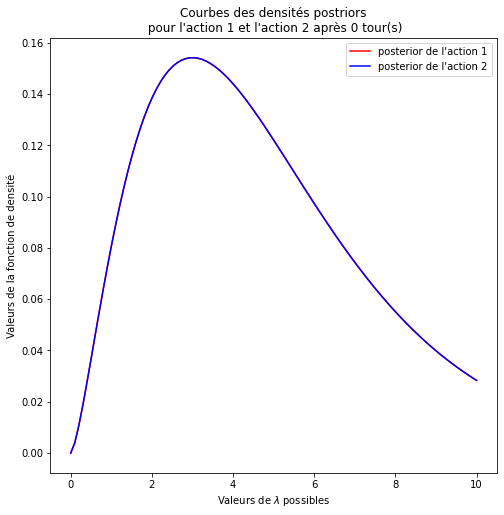
\includegraphics[scale=0.45]{posterior_tour0.png} \hfill 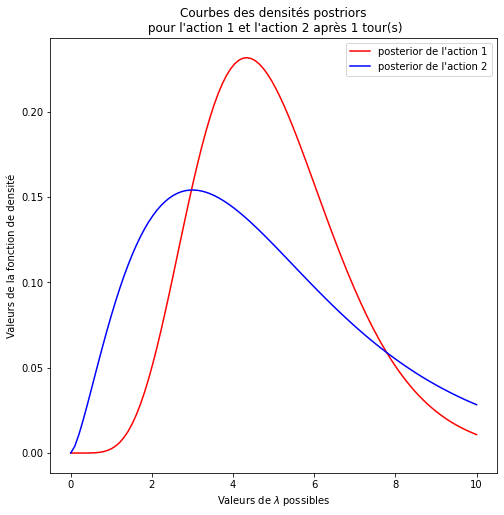
\includegraphics[scale=0.45]{posterior_tour1.png}

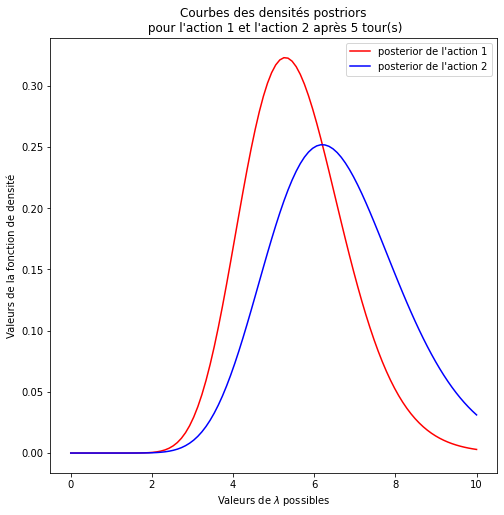
\includegraphics[scale=0.45]{posterior_tour5.png} \hfill 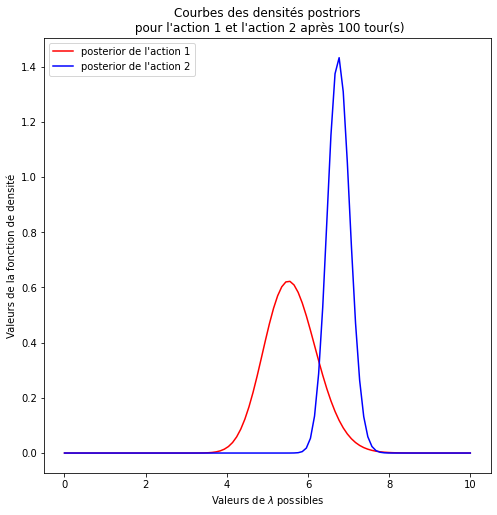
\includegraphics[scale=0.45]{posterior_tour100.png}

%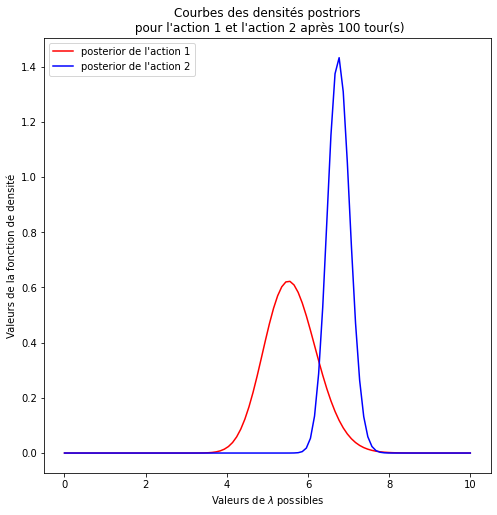
\includegraphics[scale=0.5]{posterior_tour100.png}

\end{center}
\end{figure}

\subsection{Expérimentation sur l'algorithme}

Dans cette section, on explore le comportement de l'algorithme dans diverses situations tout en s'efforçant de discuter de la sélection des priors. En effet, la loi de gamma n'ayant aucune paramétrisation la faisant corresponde à une loi uniforme, il faut faire un choix de priors qui n'est pas trivial. Pour ce faire, on supposera ici que l'on ne connaît pas les valeurs de $\lambda$ associée à chaque bras, mais que l'on connaît à tout de moins un intervalle sur lequel ils se trouvent. Dépendant des choix des priors, ces derniers sont des distributions qui peuvent couvrir bien ou non l'intervalle possibles des $\lambda,$ on suspecte que cela aura un effet sur le pseudo-regret cumulatif.\\

Pour établir une prior, il faut établir un couple $\alpha_0,\,\beta_0.$ Nous établirons plutôt un moyenne $(\mu_0)$ et une variance ($\sigma_0^2$) pour cette distribution prior et obtiendrons $\alpha_0$ et $\beta_0$ associées avec les équations (\ref{equation: alpha gamma}) et (\ref{equation: beta gamma}).

\subsection*{Remarque sur les simulations}

Dans les simulations suivantes, nous avons opté pour un $N=200,$ puisque cela offre un bon compromis entre un $N$  grand offrant un temps de calcul trop grand et un $N$ trop petit donnant lieu à des résultats biaisés par certaines instances atypique. Un $N=200$ facilite aussi la correction puisque les images peuvent être reproduites sans perdre trop de temps. Conséquemment, nous ne commenterons pas les écarts entre certaines courbes rapprochées, puisque dans d'autres simulations avec $N=1000,$ on observe que ces écarts s'atténuent ou s'inversent. Nos commentaires se feront donc sur les observations significatives dans le cas présenté $N=200$, ces dernières restaient les mêmes  ou très similaires dans le cas $N=1000.$
 
\subsubsection{Effet de la variance de la loi prior}

\subsubsection*{Expérience sur des variances trop petites}

On génère $N=200$ instances de bandits de Poisson à deux bras.\\
Pour chaque instance, les moyennes $\lambda_1, \lambda_2$ des bras sont tirées aléatoirement d'une loi uniforme continue sur l'intervalle $[0,10]$.\\
%On considérera le cas ici ou l'agent sait que les moyennes sont dans cet intervalle.\\

Pour chaque couple ($\mu_0,$ $\sigma^2_0,$) suivant:

$$(5,10),\,(5,5),\,(5,1),\,(5,1/2),\,(5,1/4)$$

On trouve $\alpha_0$ et $\beta_0$ associée à l'aide des équations $(\ref{equation: alpha gamma})$ et $(\ref{equation: beta gamma}).$
\\

On fait jouer Thompson Sampling sur les $N=200$ instances sur un horizon $T=1000.$\\
 
On trace les pseudos-regrets cumulatifs moyens avec une déviation standard au dessus (en pointillés).\\

Notons qu'ici, dans les différents couples $(\mu_0,\sigma^2_0)$ explorés, la moyenne est toujours 5 (le centre de l'intervalle [0,10]) et la variance varie (partant de 10 correspondant à la grandeur de l'intervalle et se rapetissant).\\

La figure suivante montre le résultat obtenu.

\begin{figure}[H]
\label{figure: variance petite}
\caption{Comparaisons de la performance selon des priors de variances plus petites}
\begin{center}
%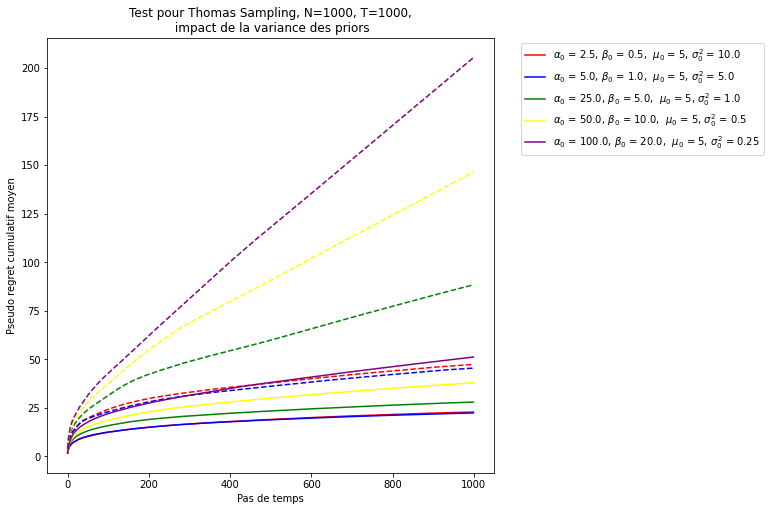
\includegraphics[scale=0.5]{etude_variance_petite.png} 
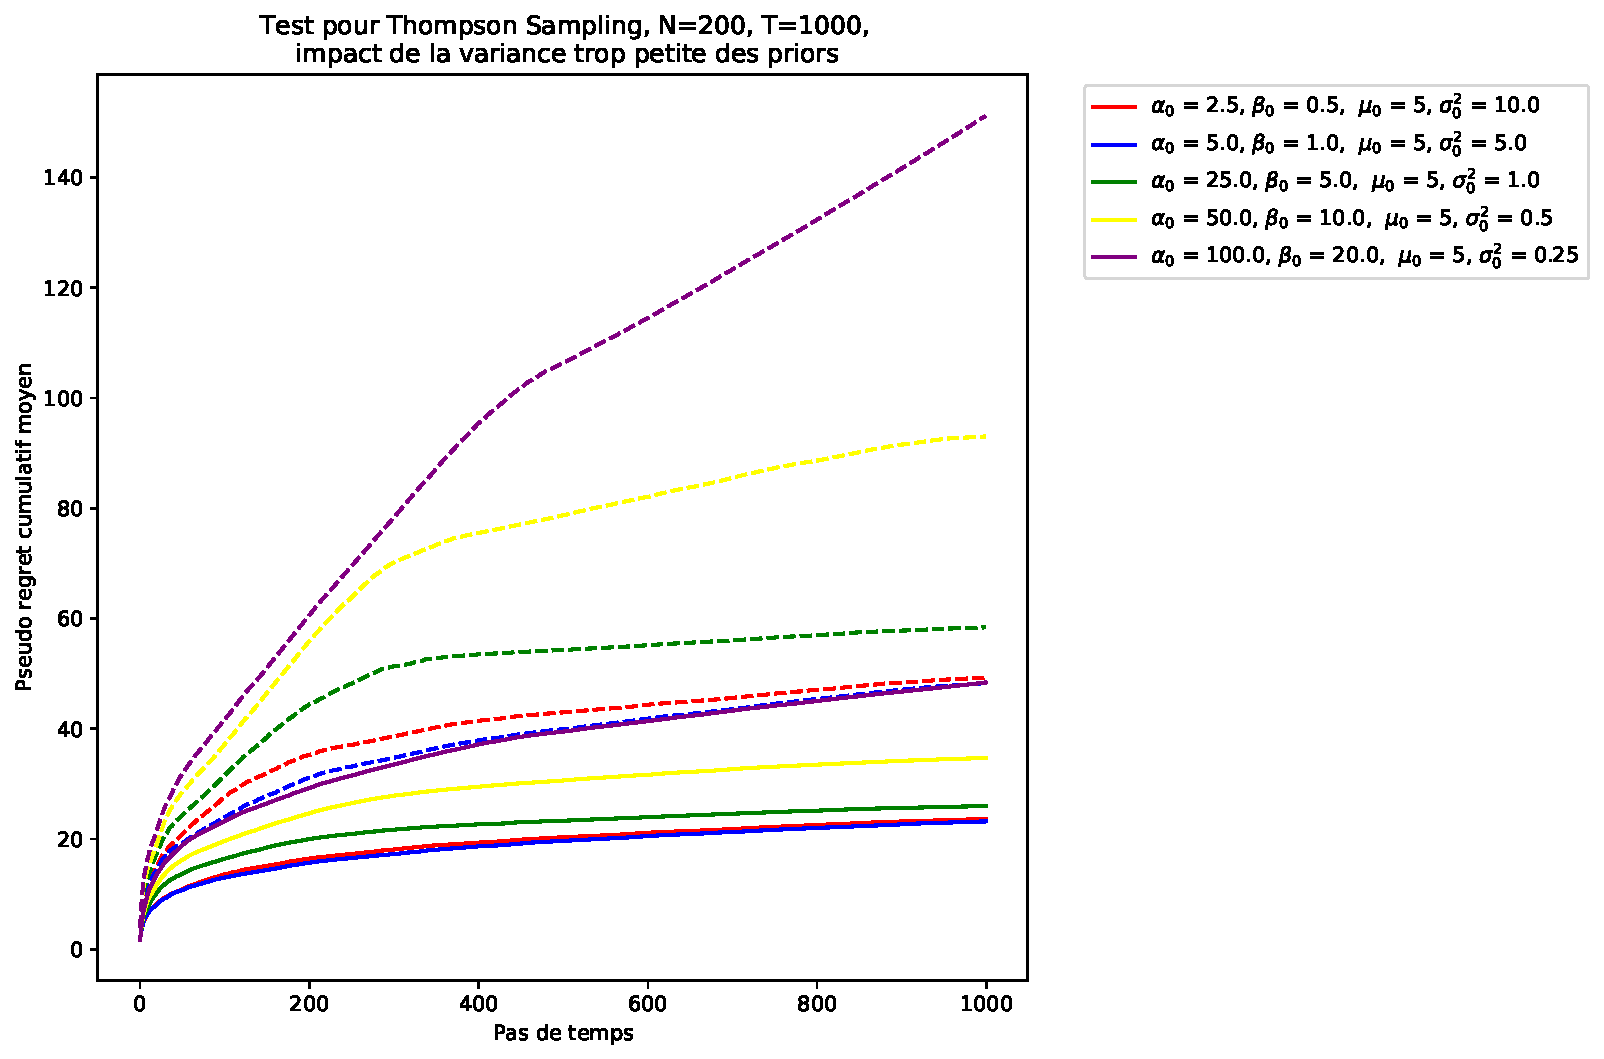
\includegraphics[scale=0.5]{variance_trop_petites_N=200.pdf} 
\end{center}
\end{figure}

On remarque que si la distribution prior est choisie avec une variance trop petite, la distribution prior ne couvre pas suffisamment bien l'intervalle $[0,10]$ des valeurs possibles de $\lambda$ et cela semble se traduire par une augmentation du pseudo-regret cumulatif moyen. On remarque qu'il semble y avoir un certaine tolérance sur des variations de $\sigma^2_0$ qui ne changent pas significativement la courbe du pseudo-regret cumulatif moyen. 

\subsubsection*{Expérience sur des variances trop grandes}

Même méthode que l'expérience 1, mais sur les couples $(\mu_0,\sigma^2_0)$ suivants.

$$(5,10),\,(5,20),\,(5,50),\,(5,100),\,(5,1000)$$

La moyenne des priors est toujours le centre de l'intervalle $[0,10],$ la variance varie (partant de 10 correspondant à la grandeur de l'intervalle et se grandissant).\\

La figure suivante montre le résultat obtenu.

\begin{figure}[H]
\label{figure: variance petite}
\caption{Comparaisons de la performance selon des priors de variances plus grandes}
\begin{center}
%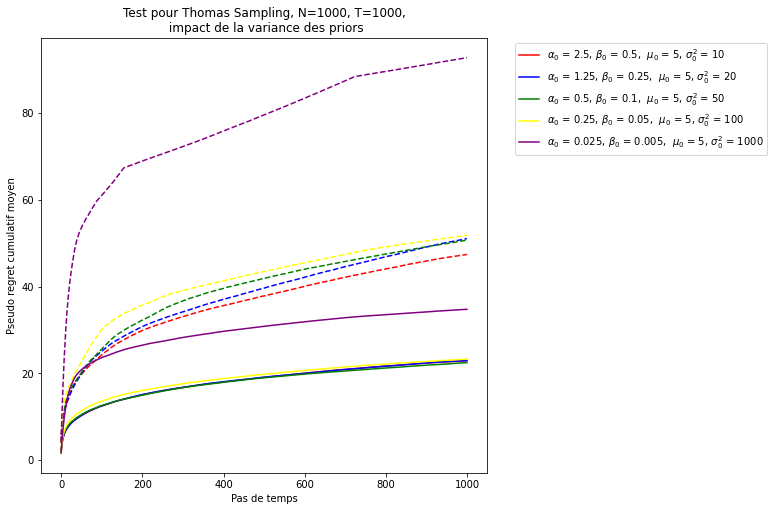
\includegraphics[scale=0.5]{etude_variance_grande.png} 
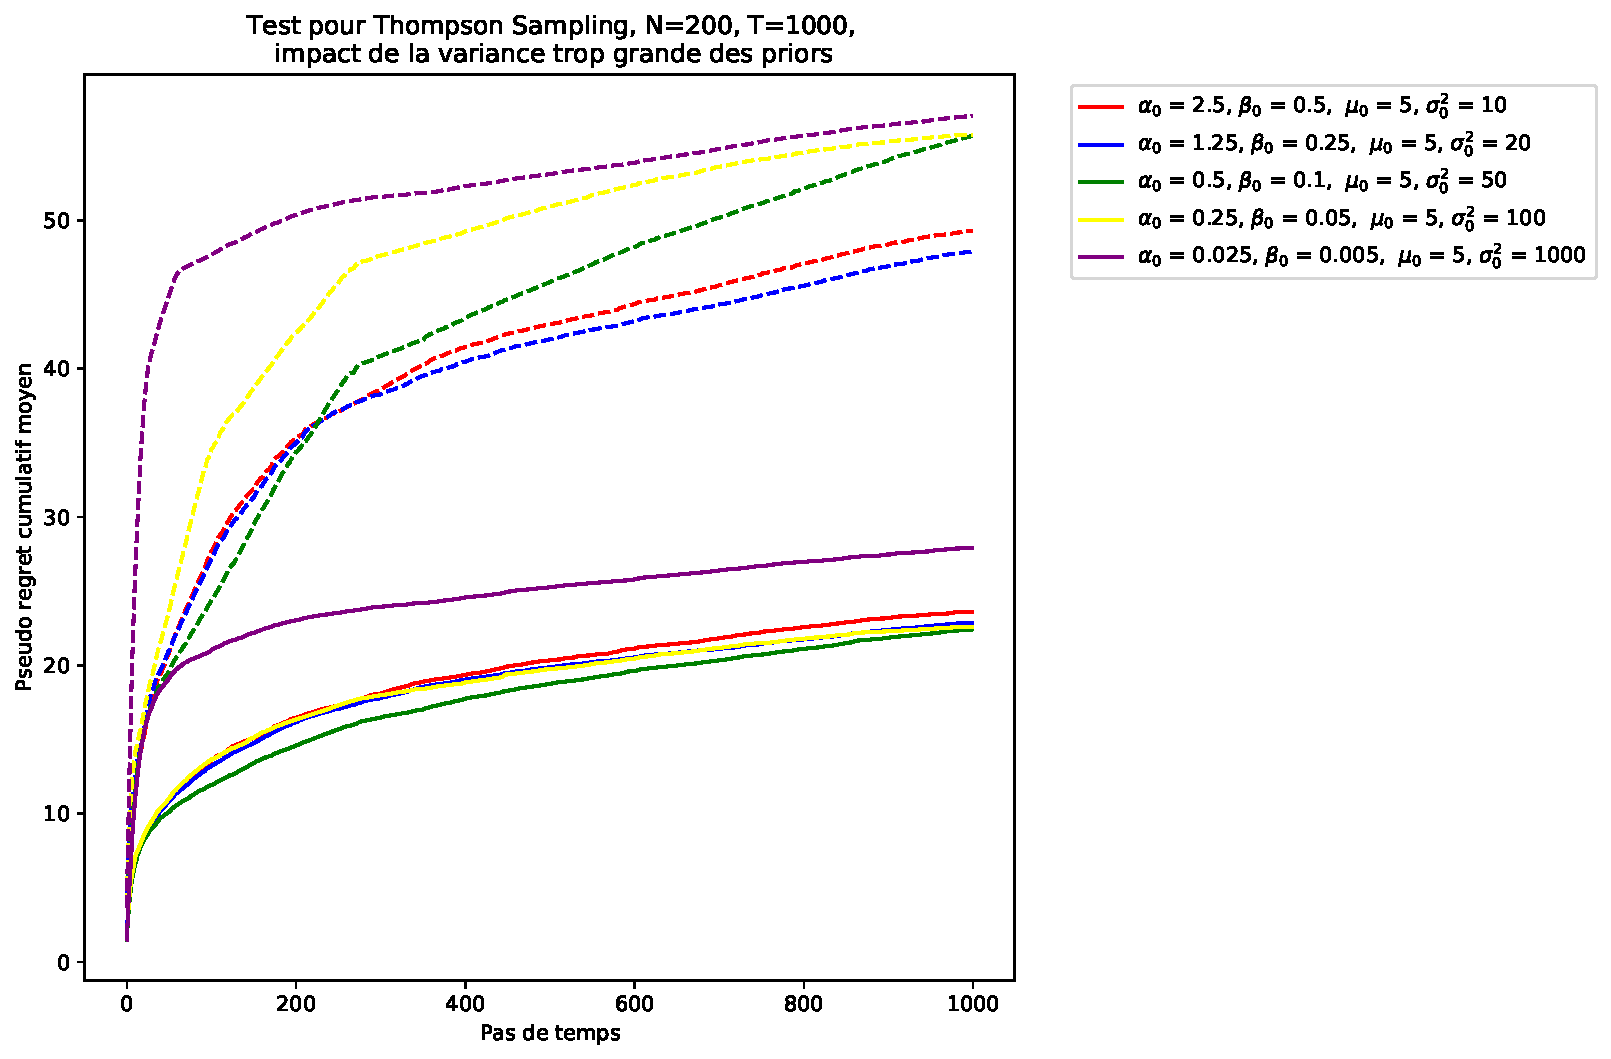
\includegraphics[scale=0.5]{variance_trop_grande_N=200.pdf}
\end{center}
\end{figure}

On peut voir qu'une variance légèrement trog grande n'aura pas beaucoup d'effet sur le regret cumulatif moyen, par contre, une variance excessivement trop grande peut en avoir un considérable. Dans ce cas ($\sigma^2_0=1000$), la distribution prior sur-couvre grandement l'intervalle [0,10] des valeurs possibles de $\lambda.$ Conséquemment, possiblement que les distributions posteriors ne se concentrent pas suffisamment rapidement pour pouvoir bien cerner les moyennes $\lambda_1$ et $\lambda_2$ des distributions de Poisson des bras.

\subsubsection{Effet de la moyenne de la loi prior avec variance <<bonne>>}

Pour bien pouvoir faire varier les moyennes de la prior choisi, on va ici considérer une situation analogue aux deux premières expériences, mais où l'intervalle sur lequel sont choisis les moyennes $\lambda_1, \lambda_2$ est $[10,20]$ au lieu de $[0,10].$ On effectue la même expérience que si haut, sur les couples  $(\mu_0 ,\sigma^2_0)$ qui suivent.


$$(5,10),\,(12,10),\,(15,10),\,(17,10),\,(25,10)$$

La variance de la prior est fixe égale à la longueur de l'intervalle des valeurs possibles de $\lambda.$\\ 

On obtient la figure suivante

\begin{figure}[H]
\label{figure: moyenne décalée 1}
\caption{Comparaisons de la performance selon des priors de variances égale à la longueur de l'intervalle et de moyennes variables.}
\begin{center}
%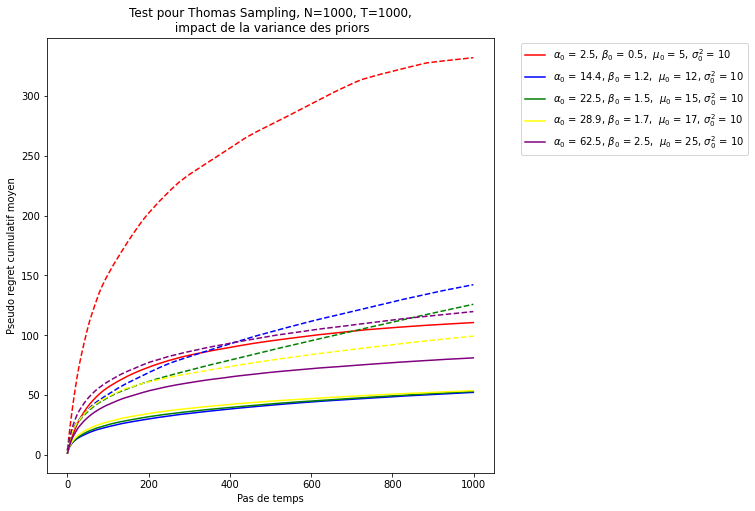
\includegraphics[scale=0.5]{etude_moyenne_decale_var10.png} 
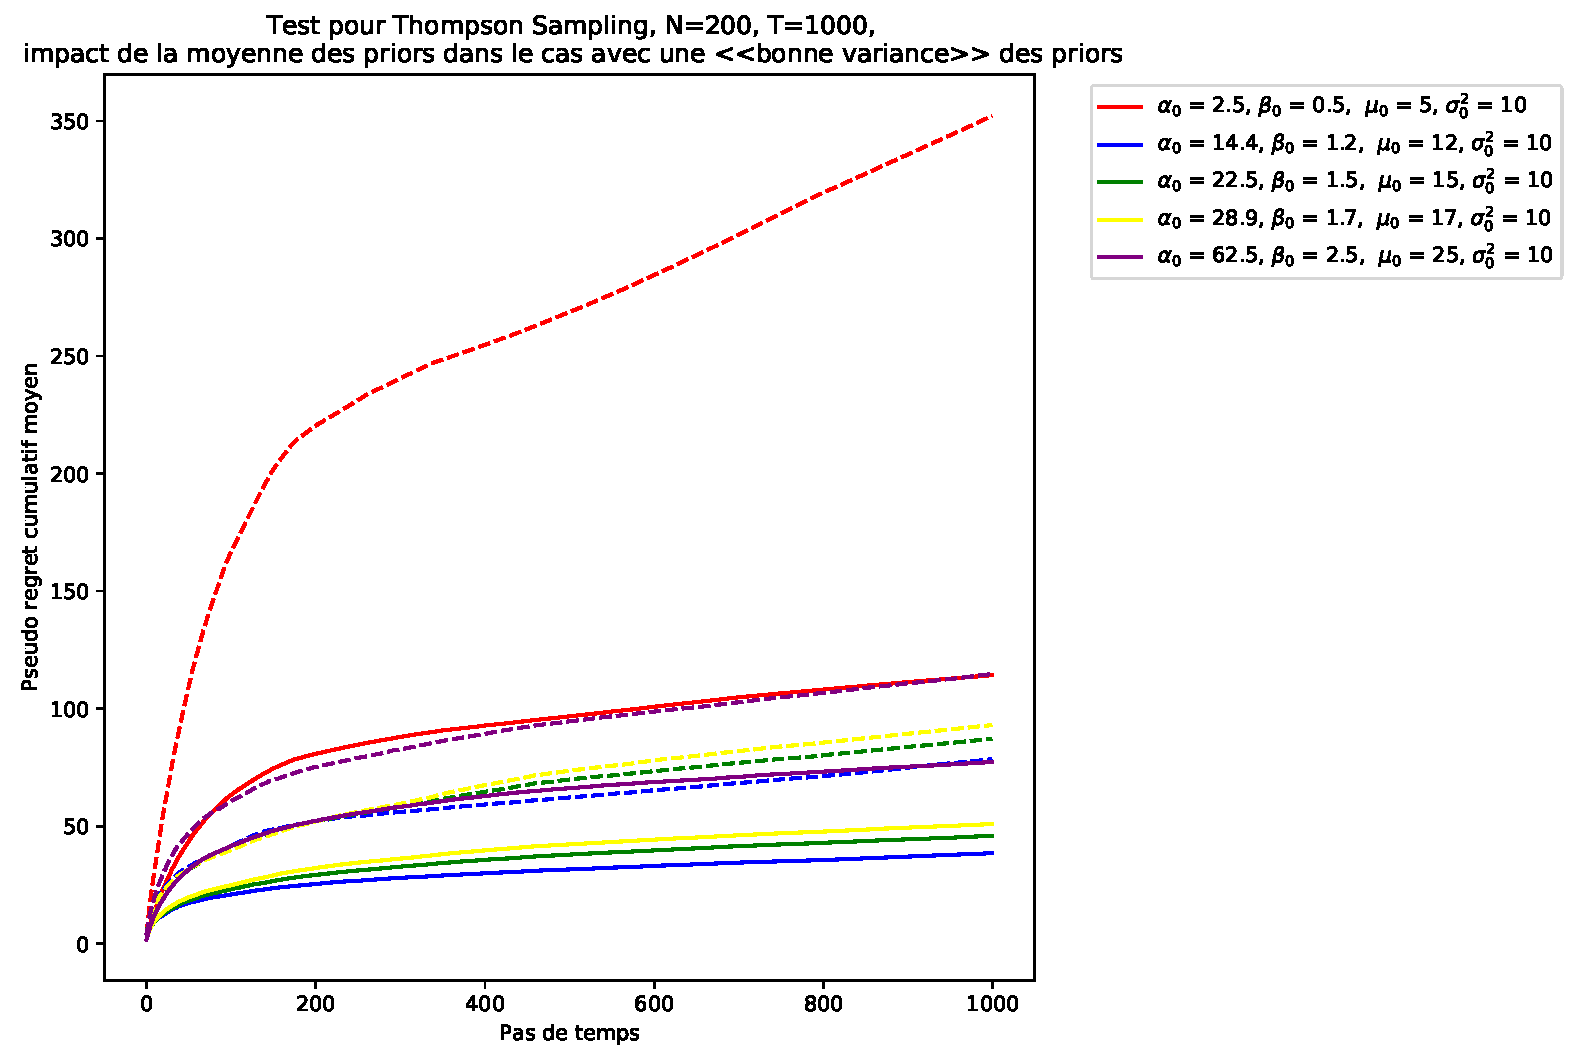
\includegraphics[scale=0.5]{moyenne_decentree_variance_bonne_N=200.pdf}
\end{center}
\end{figure}

On remarque que si la moyenne du prior est fortement décalée du centre de l'intervalle $[10,20]$, cela aura un effet sur la performance de l'algorithme, notamment le cas où $\mu_0=5.$ Lorsque la moyenne $\mu_0$ reste dans l'intervalle $[10,20],$ il semble que le fait que la variance soit bonne (distribution prior qui couvre bien l'intervalle) fait en sorte que l'algorithme reste bon même si $\mu_0$ n'est pas centré.   

\subsubsection{Effet de la moyenne de la loi prior avec variance plus petite}

Même expérience que précédemment, mais avec les couples $(\mu_0,\sigma^2_0)$ qui suivent.

$$(9,3),\,(12,3),\,(15,3),\,(17,3),\,(21,3)$$

Cette fois, la variance est plus petite (3).\\

On obtient la figure suivante

\begin{figure}[H]
\label{figure: moyenne décalée 1}
\caption{Comparaisons de la performance selon des priors de variances égalent à 3 et moyennes variables.}
\begin{center}
%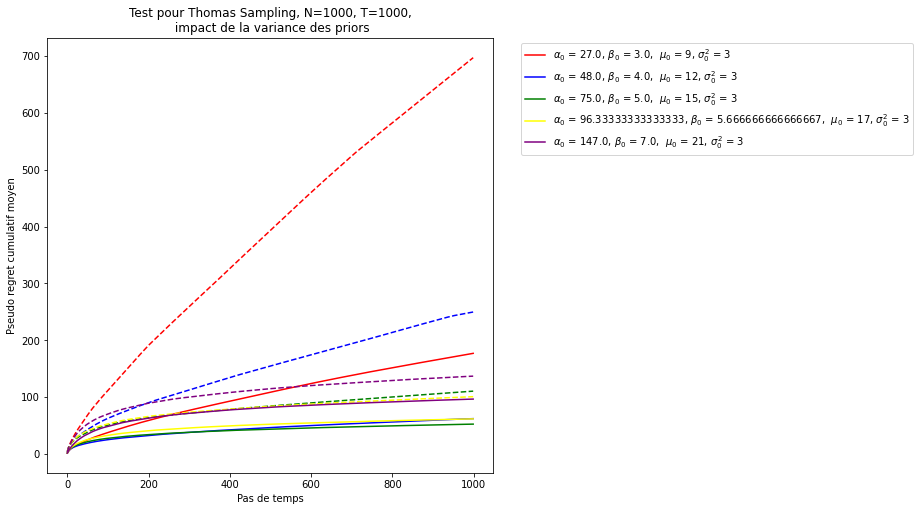
\includegraphics[scale=0.5]{etude_moyenne_decale_var3.png} 
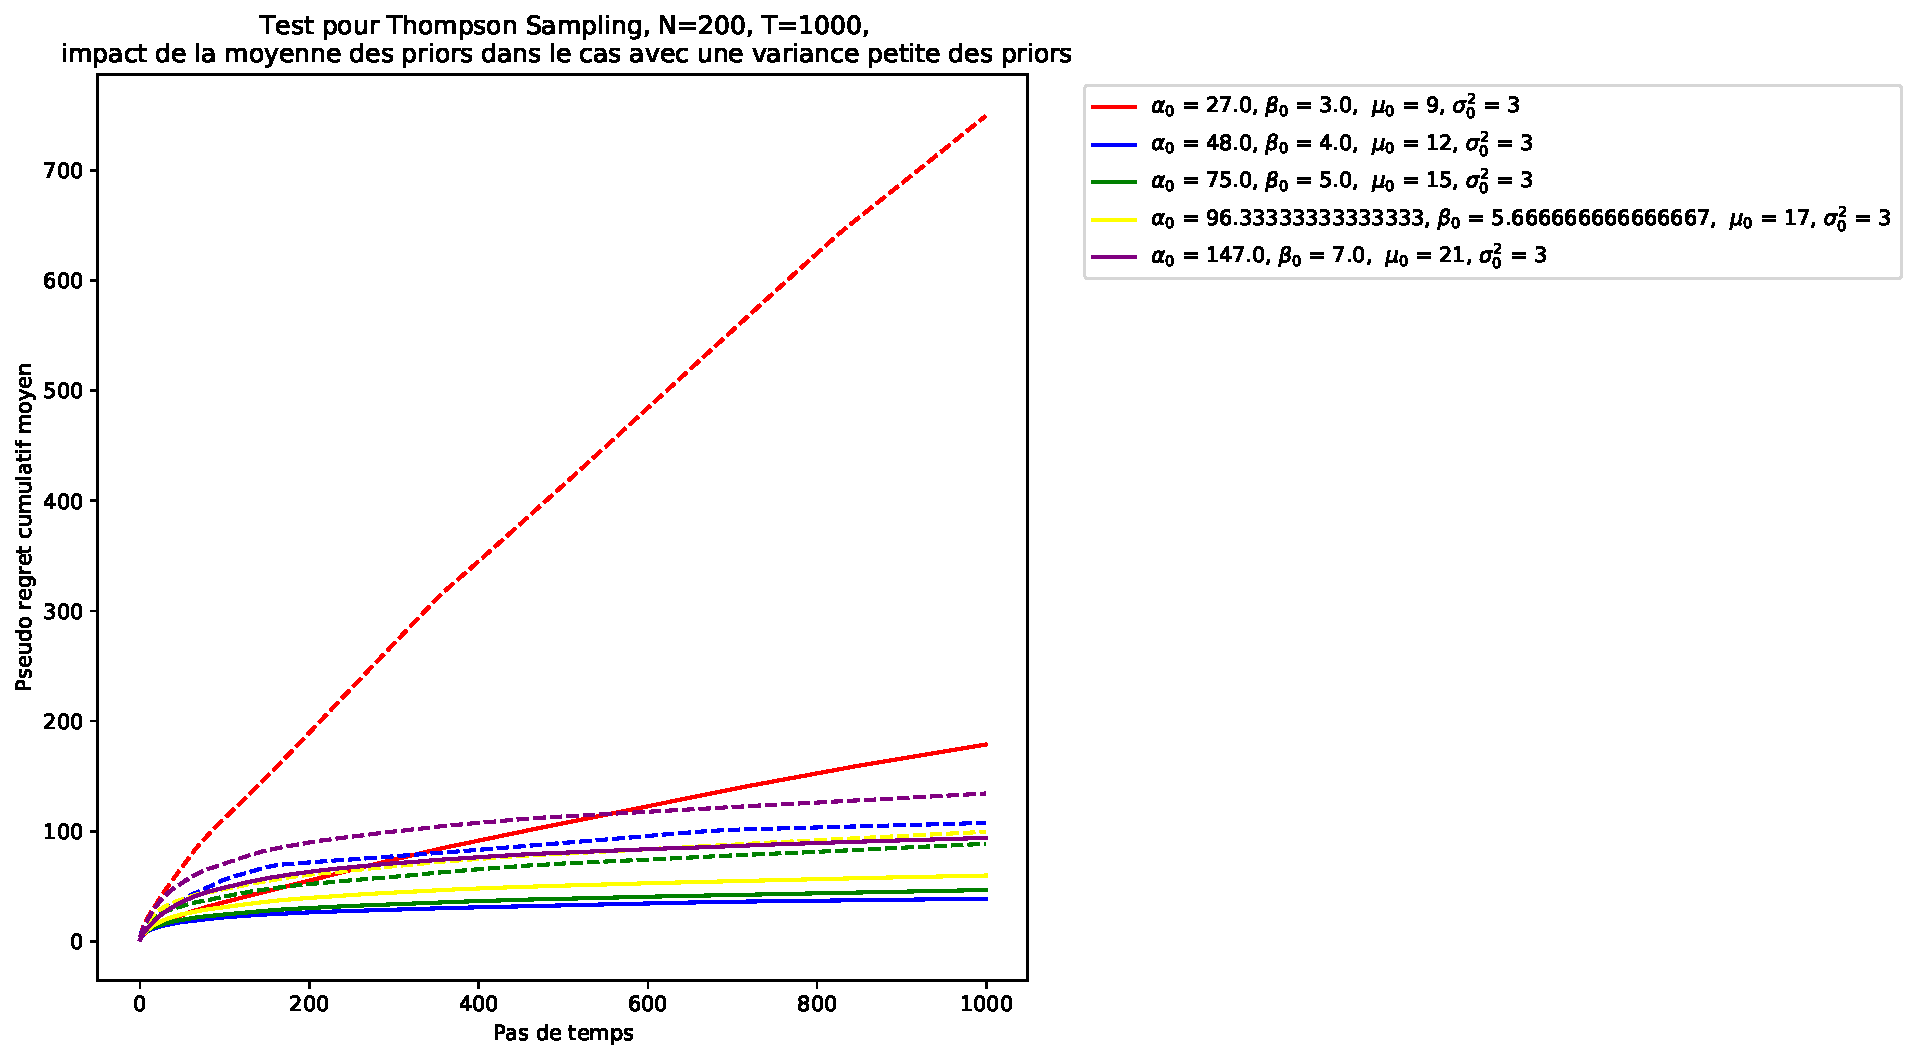
\includegraphics[scale=0.5]{moyenne_decentree_variance_petite_N=200.pdf}
\end{center}
\end{figure}

On voit qu'ici, avec une variance des priors plus petite, un même décalage de la moyenne $\mu_0$ par rapport au centre de l'intervalle semble être plus coûteux que dans l'expérience précédente. D'ailleurs, le cas $\mu_0=9$ semble en être un bon exemple car il atteint une regret cumulatif moyen final plus élevé que le cas $\mu_0=5$ dans le cas où la variance était de 10 (voir expérience précédente). Conséquemment, si l'information que l'on a à priori sur les $\lambda$ (intervalle de possibilité) n'est pas bonne pour fixer les priors, lancer un tel algorithme avec une variance trop petite peut avoir un impact sur la performance, notamment si par malchance on choisit un prior avec $\mu_0$ décalé du centre du réel intervalle des valeurs possibles de $\lambda.$\\

En conclusion, à la lumière des simulations effectuées, les priors semblent devoir être choisis pour couvrir raisonnablement bien l'intervalle des valeurs possibles de $\lambda.$ On pourrait suggérer de prendre la distribution prior telle que $\mu_0$ est le centre de l'intervalle et $\sigma^2_0$ la longueur de l'intervalle. Selon nos simulations (notamment avec $N=1000$ non-présenté ici), cela semble être un choix raisonnable.

\section{No 4}

\subsection{Contexte}

On considère le cas d'un bandit contextuel à $M$ actions avec un espace de contexte $S.$ Dans ce <<setting>>, à chaque temps $t,$ l'agent observe un contexte $s_t$ à partir duquel il doit sélectionner une actions $m_t\in{1,2,\ldots,M}$ et observer un reward $r_t=f_{m_t}(s_t)+\eta_t$ où $\eta_t\sim\mathcal{N}(0,\sigma^2).$ La figure suivante montre une situation hypothétique avec un contexte $S=[0,1]$ et $M=2$ actions. 

\begin{figure}[H]
\caption{Illustration d'un contexte de bandit contextuel}\label{figure: contexte}
\begin{center}
%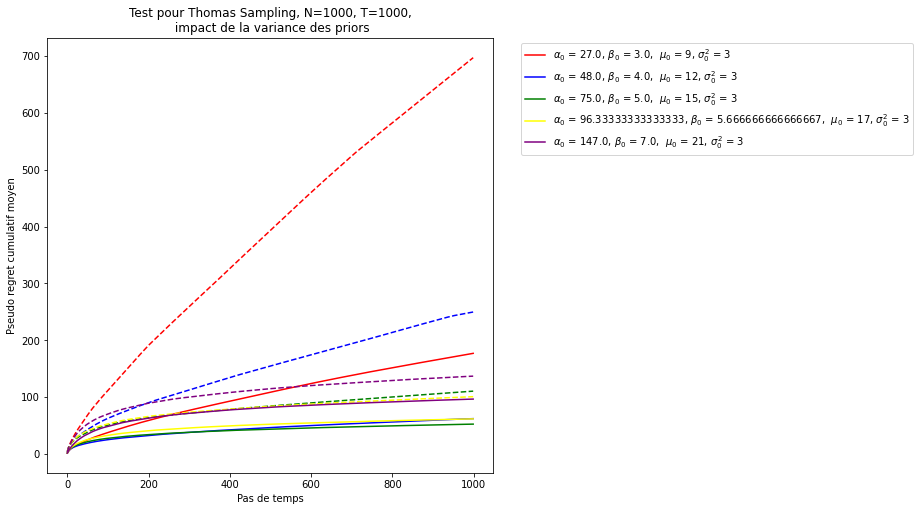
\includegraphics[scale=0.5]{etude_moyenne_decale_var3.png} 
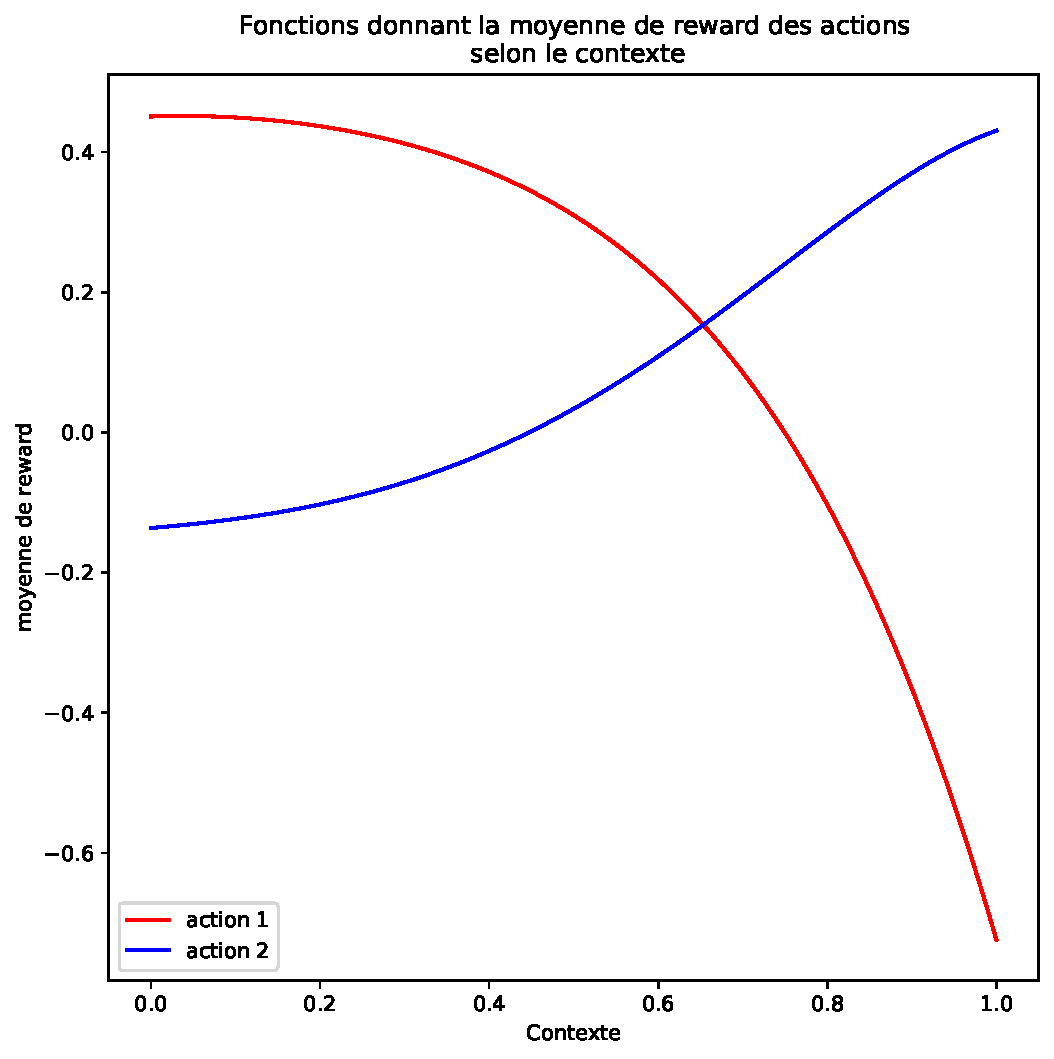
\includegraphics[scale=0.5]{image_contexte_no4.pdf}
\end{center}
\end{figure}

On désire définir l'algorithme Kernel Thompson Sampling dans cette situation. En s'inspirant de \textit{Durand, A., Maillard, O. A., et Pineau, J. (2018)}, on arrive au pseudo-code suivant.
  
\subsection{Pseudo-code}

Entrées de l'algorithme:\\

\begin{itemize}
\setlength\itemsep{0.2cm}

\item
Pour $1\leq t \leq T$ 

\begin{itemize}
\item
Pour chaque bras $m=1,2,\ldots,M$

\begin{itemize}
\item
Calculer les moyennes posteriors $\widehat{f}_{t-1,m}=(f_{\lambda_t,t-1,m}(s))_{s\in\mathbb{S}}$

\item
Calculer la covariance posteriors $\widehat{\Sigma}_{t-1,m} = \dfrac{\sigma^2_{+,t-1}}{\lambda_t}\left(k_{\lambda_t,t-1}(s,s')\right)_{(s,s')\in\mathbb{S}}$

\item
échantillonner $\widetilde{f}_{t,m}=\mathcal{N}\left(\widehat{f}_{t-1,m}\,;\,v^2_t\,\widehat{\Sigma}_{t-1,m}\right)$

\end{itemize}
\item
observer un contexte $s_t\in\mathbb{S}$

\item
$m_t = \underset{m}{\mathrm{argmax}} \tilde{f}_{t,m}(s) $

\item
Jouer l'action $m_t$

\item
Observer un reward: $y_t=f_{m_t}(s_t)+\eta_t$

\end{itemize}

\end{itemize}

\subsubsection{Détails de l'implémentation}

Pour simplifier l'algorithme, on lui passera simplement $\sigma$ comme valeur de $\sigma^2_{+,t-1}$ et on prendra $\lambda=\sigma^2$ étant donner que les fonctions de rewards seront des fonctions polynomiales dont les coefficients sont les éléments d'un vecteur $\theta$ de norme 1. \textbf{Aussi, notons que le pseudo-code précédent conserve la forme de l'article, alors que pour l'implémentation, on initialisera $\widehat{f}$ et $\widehat{\Sigma}$ pour chaque bras avant le premier tirage de $\tilde{f},$ ensuite, à la fin de chaque itération, $\widehat{f}$ et $\widehat{\Sigma}$ seront calculés avec l'aide d'un <<Gaussian Process Regressor>>}. Aussi, l'espace de contexte $\mathcal{S}$ s'est vue discrétisée en $\mathbb{S}$ pour faciliter l'implémentation. De plus, dans le Gaussian Process Regressor, nous avons utilisé un noyau RBF avec une bandwidth de 1 dans l'expérience ci-dessous. Finalement, comme écrit dans l'article de référence au sujet des performances en pratiques, nous avons choisi un $v_t^2$ de 1. 

\subsection{Expérimentation}

On a joué l'algorithme sur un horizon $T=100$ sur une instance des deux bandits dont le graphe des rewards moyen est présenté à la figure \ref{figure: contexte}. Les figures suivantes montrent les fonction $\widehat{f}$ pour chacune des deux actions selon le nombre de tours joués.

\begin{figure}[H]
\caption{Évolution des posteriors}
\label{figure: évolution des posteriors}
\begin{center}

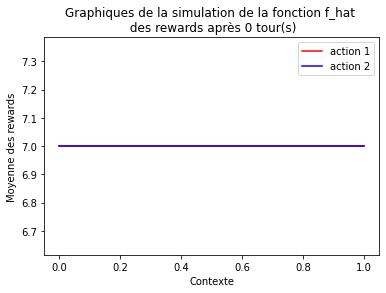
\includegraphics[scale=0.45]{KTS-0-tour.png} \hfill 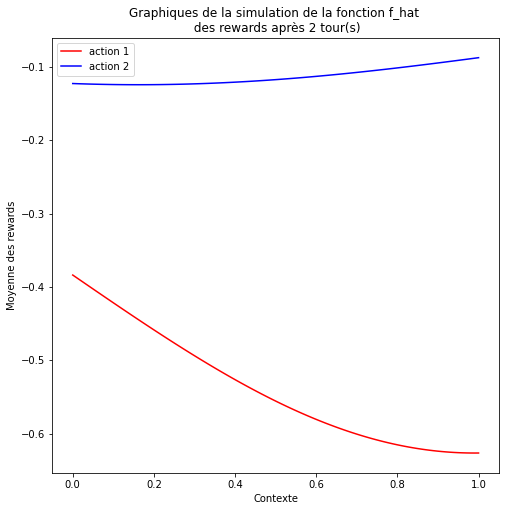
\includegraphics[scale=0.45]{KTS-2-tours.png}

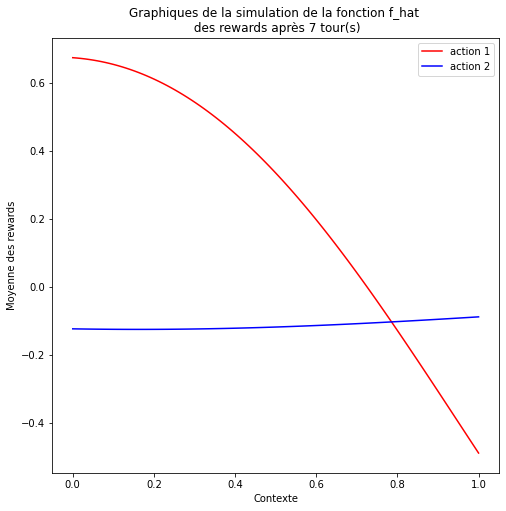
\includegraphics[scale=0.45]{KTS-7-tours.png} \hfill 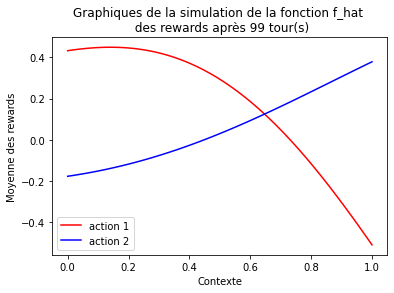
\includegraphics[scale=0.45]{KTS-99-tours.png}

%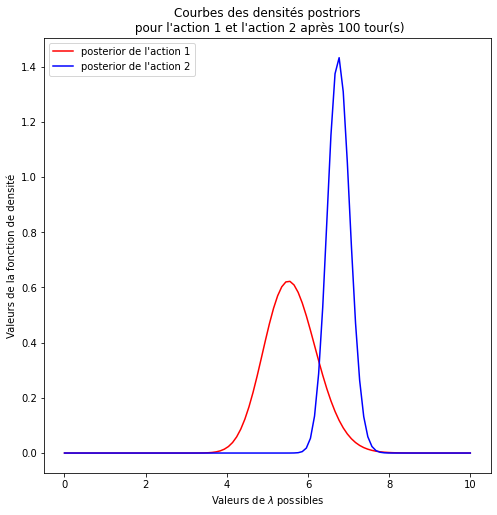
\includegraphics[scale=0.5]{posterior_tour100.png}

\end{center}
\end{figure}

On peut voir que l'algorithme estime de mieux en mieux les fonctions des moyennes des rewards à mesure qu'il joue. On voit qu'à la fin, le graphe estimé est très près des vrais graphiques représentant les actions montrés à la figure \ref{figure: contexte}.\\

Voici le pseudo regret cumulatif pour la même expérience

\begin{figure}[H]
\label{figure: pseudo KTS}
\caption{Performance de Kernel Thompson Sampling}
\begin{center}
%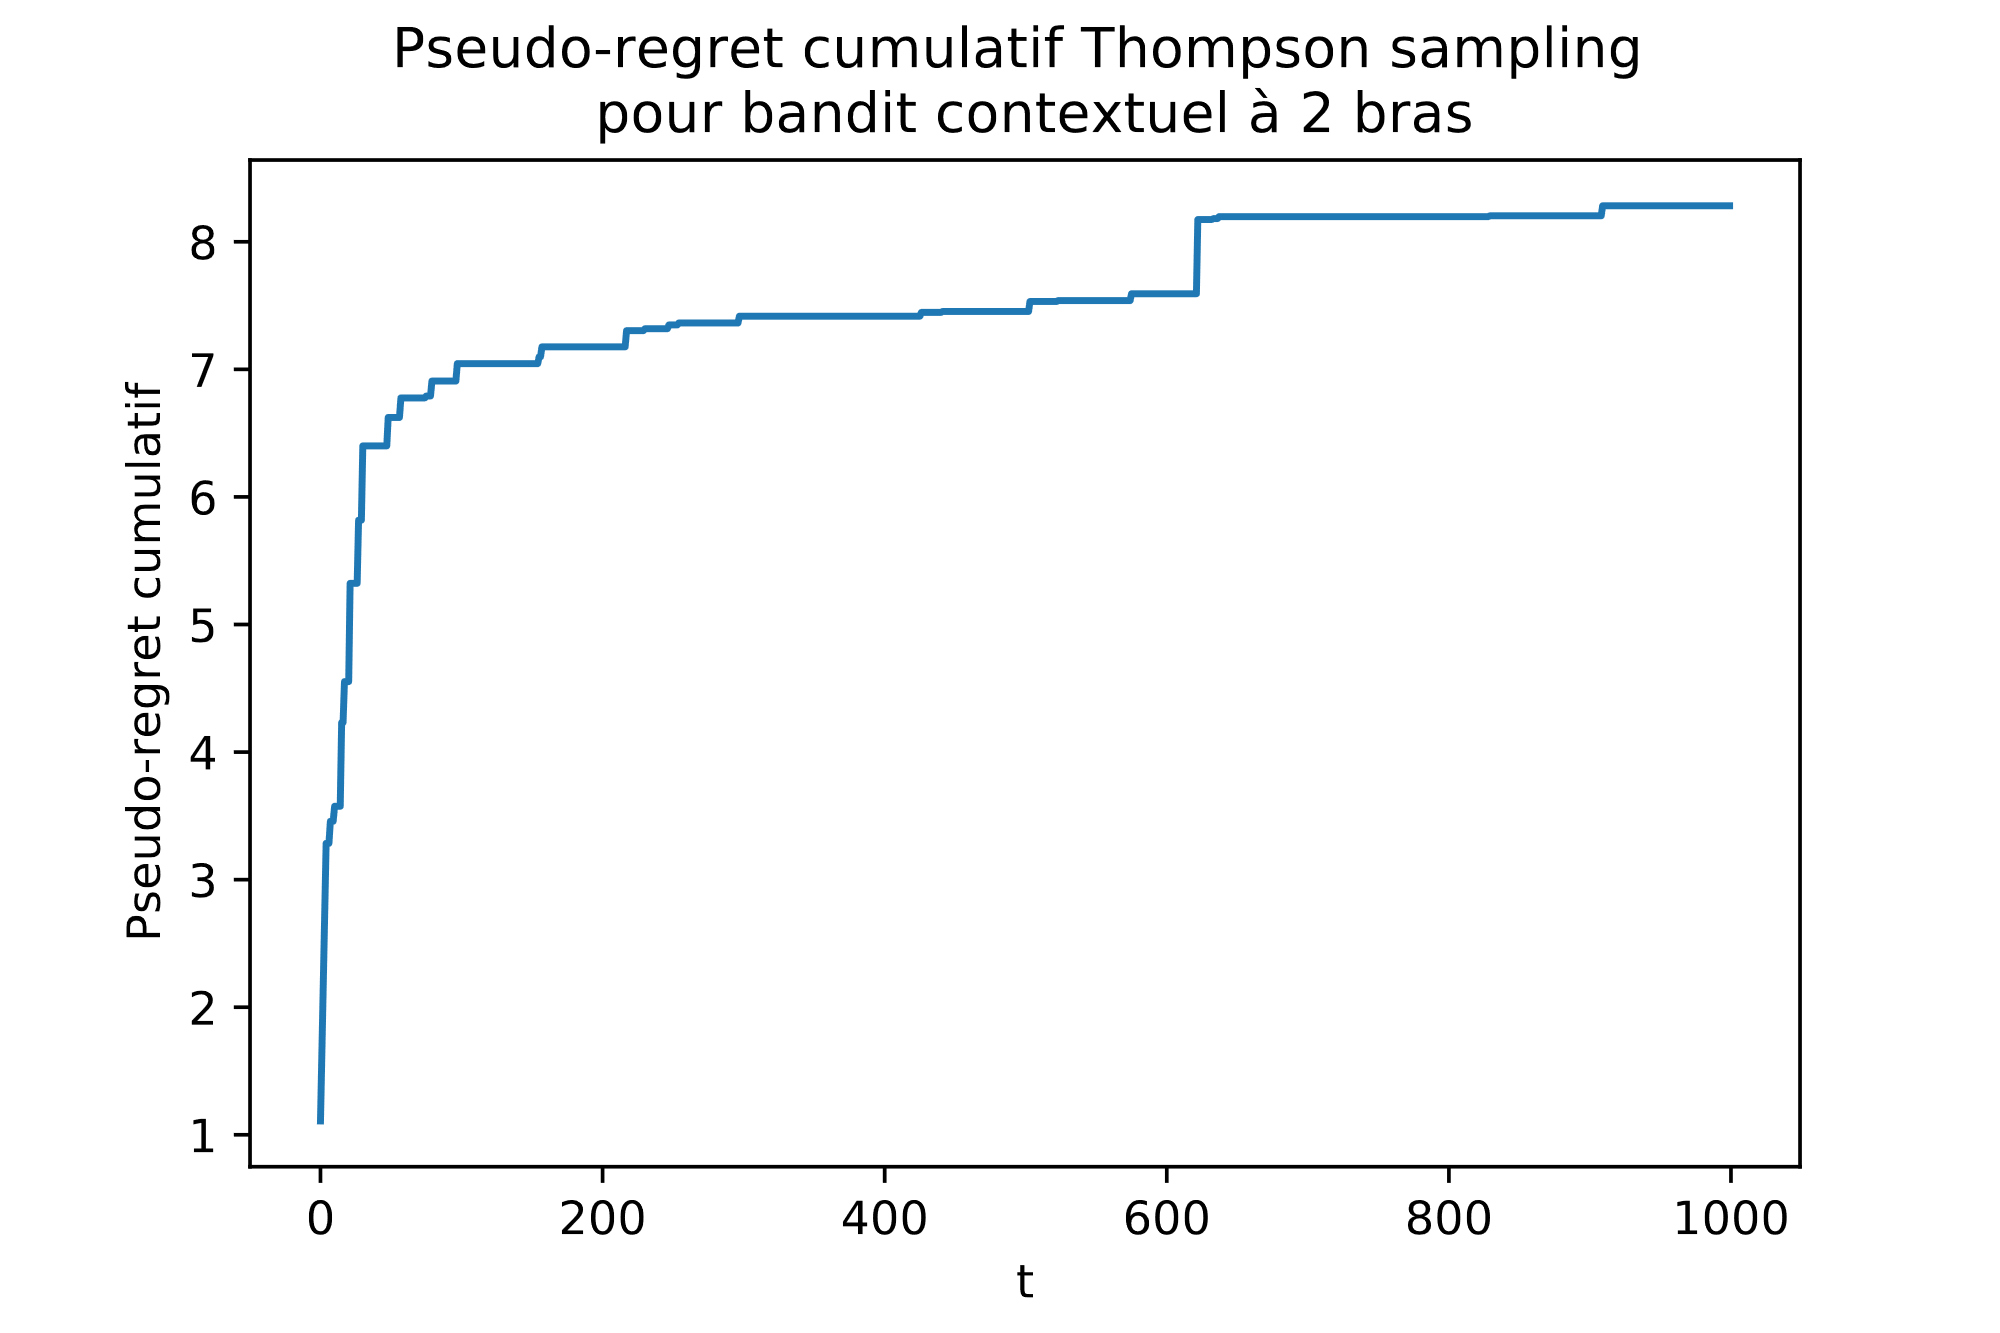
\includegraphics[scale=0.2]{pseudo-KTS.png}
\end{center}
\end{figure}

On voit un comportement typique pour ce type d'algorithme, c'est-à-dire que celui-ci cumule du regret passablement souvent au début à mesure qu'il cumule de l'information pour ensuite être bien en selle pour choisir presque tout le temps l'action optimale. On peut voir dans le graphique certaines brisures suivies de plateaux même pour de grands $t$, ces brisures sont potentiellement associées à des moments où le contexte $s$ donné à l'agent était problématique, étant près de l'abscisse d'intersection entre les deux courbes d'action, ce qui peut produire un mauvais choix de l'action optimale. 

\end{document}
